
%\documentclass[aspectratio=169]{beamer}
\documentclass{beamer}
\usetheme{Warsaw}
\usepackage{graphicx}
\usepackage{color}
\usepackage{listings}
\definecolor{dkgreen}{rgb}{0,0.6,0}
\definecolor{gray}{rgb}{0.5,0.5,0.5}
\definecolor{mauve}{rgb}{0.58,0,0.82}
\usepackage{amssymb}
\usepackage{amsthm}
\usepackage{amsmath}
\usepackage{amsopn}
\usepackage{hyperref}
\definecolor{codegreen}{rgb}{0,0.6,0}
\definecolor{codegray}{rgb}{0.5,0.5,0.5}
\definecolor{codepurple}{rgb}{0.58,0,0.82}
\definecolor{backcolour}{rgb}{0.95,0.95,0.92}
 \usepackage[version=4]{mhchem}
\lstdefinestyle{mystyle}{
    backgroundcolor=\color{backcolour},   
    commentstyle=\color{codegreen},
    keywordstyle=\color{magenta},
    numberstyle=\tiny\color{codegray},
    stringstyle=\color{codepurple},
    basicstyle=\footnotesize,
    breakatwhitespace=false,         
    breaklines=true,                 
    captionpos=b,                    
    keepspaces=true,                 
    numbers=left,                    
    numbersep=5pt,                  
    showspaces=false,                
    showstringspaces=false,
    showtabs=false,                  
    tabsize=2
}
\lstset{style=mystyle}
 \usepackage{pst-node,graphicx}
%\definecolor{mygreen}{RGB}{88, 102, 61}
\definecolor{myblue}{RGB}{51, 122, 153}
\definecolor{mygrey}{RGB}{ 216, 229, 215}
\definecolor{myred}{RGB}{198, 99, 59}
\definecolor{mywhite}{RGB}{255, 251, 244}
\definecolor{myolive}{RGB}{143, 163, 132}
\setbeamercolor{alerted text}{fg=orange}
\setbeamercolor{background canvas}{bg=mywhite}
\setbeamercolor{block title}{bg=myblue}
\setbeamercolor{normal text}{bg=mygrey,fg=black}
\setbeamercolor{palette sidebar primary}{use=normal text,fg=normal text.fg}
\setbeamercolor{palette sidebar quaternary}{use=structure,fg=structure.fg}
\setbeamercolor{palette sidebar secondary}{use=structure,fg=structure.fg}
\setbeamercolor{palette sidebar tertiary}{use=normal text,fg=normal text.fg}
\setbeamercolor{section in sidebar}{fg=brown}
\setbeamercolor{section in sidebar shaded}{fg=grey}
\setbeamercolor{separation line}{}
\setbeamercolor{sidebar}{bg=red}
\setbeamercolor{sidebar}{parent=palette primary}
\setbeamercolor{structure}{bg=black, fg=myblue}
\setbeamercolor{subsection in sidebar}{fg=brown}
\setbeamercolor{subsection in sidebar shaded}{fg=grey}
\setbeamercolor{title}{fg=white}
\setbeamercolor{titlelike}{fg=white}
\usepackage{epstopdf} 


\title{ Lunar Refueling Station}
\author{Leticia Damian \& Josh Lucas \& Rowan Ranjbar }
\institute[CSUSM] % (optional)
{
  \inst{1}%
  Dept. of Physics\\
  California State University San Marcos
}
 
\date % (optional){\today}

\begin{document}
 
\frame{\titlepage}


\begin{frame}{Temperature variation on lunar south pole}
Due to the sunlight being perpetually on the horizon the variations in illumination and temperature at the lunar south pole are functions of the incident sunlight as well as the topography, with smaller effects due to the moons distance from the sun and location in orbit around Earth \cite{Williams}.
\end{frame}





\begin{frame}{Temperature variation on lunar south pole}
 \begin{center}
             \includegraphics[width=\textwidth]{LunarTempmaxavg.eps}   
      \end{center}  
 The temperature vary from a average high of $213K $ and a low of $50K$.
 Despite a larger area of the Lunar south pole being permanently shadowed than the north, the topography results in increased illumination on the slopes of ridges than the northern pole.\cite{Williams}\cite{Hayne}.
\end{frame}


\begin{frame}{Sun Position from Areas at Lunar South Pole}


 \begin{center}
             \includegraphics[width=.85\textwidth]{Illum.eps}   
      \end{center}  

\end{frame}
\begin{frame}{Solar Power}
The spectrum of light emitted by the sun is different on Earth compared to space due to the Earth's atmosphere filtering of  wavelengths. Panels for Earth use are designed and calibrated differntly than those used for space\cite{Liebert} \cite{Mcevoy}.  
 \begin{center}
             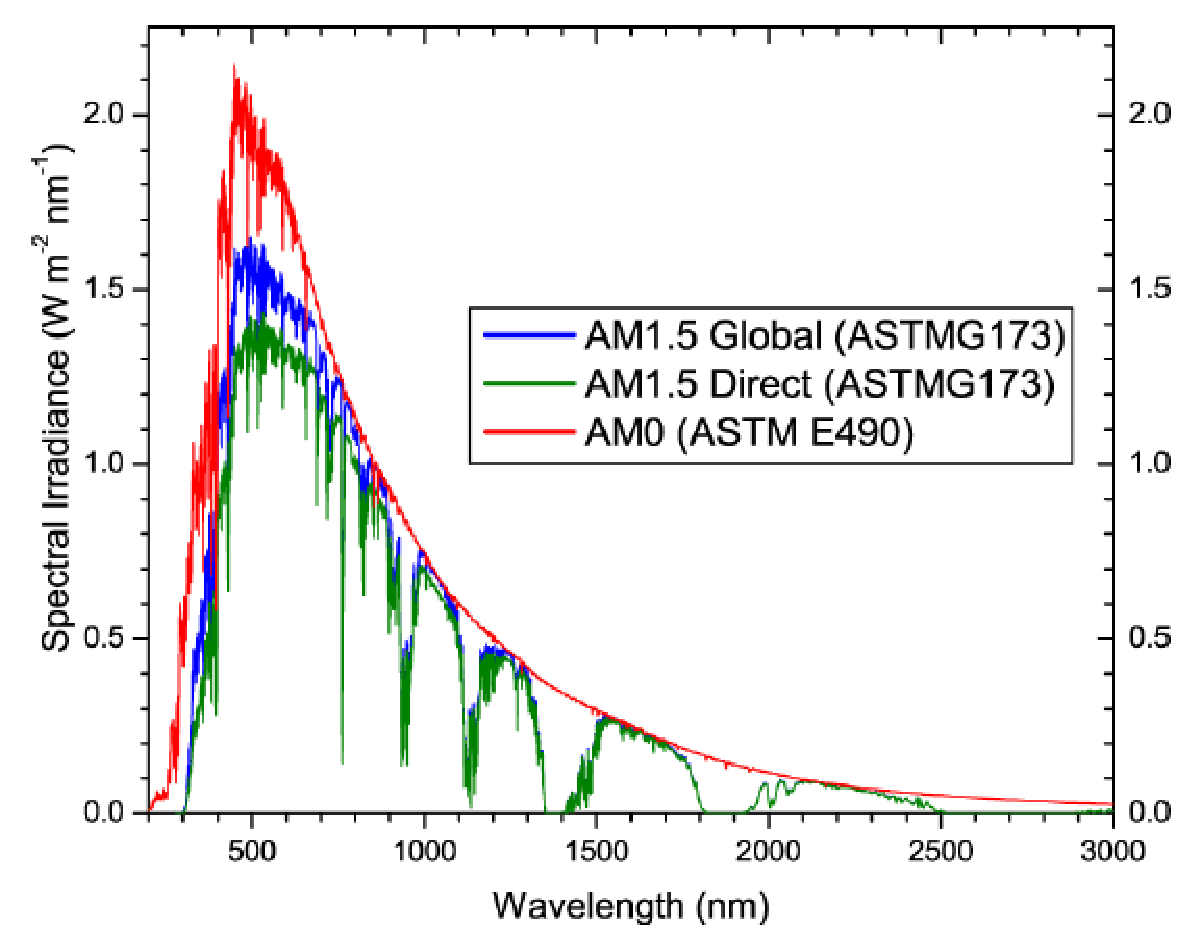
\includegraphics[width=.68\textwidth]{AM0.eps}   
      \end{center}  

\end{frame}

\begin{frame}{Solar Cells in Space}
The cells themselves need to be optimized for the change in solar intesity and the operating tempertures. GaAs has been shown to have better temperature stability and radiation resistance\cite{Mcevoy}.\\
The amount of power that can be generated by a solar cell is related to its operating temperature, which is fairly linear from $173 K - 373K$ \cite{Mcevoy}.\\ Tests conducted by Nasa simulating near earth and a colder Jupiter distance showed increased efficiency ($14-15\%\ vs\ 10-11\%  $) at the colder temperatures despite the lower levels of illumination\cite{Liebert}.
\end{frame}

\begin{frame}{Solar Power Generation}
By taking adavtage of the areas with perpetual sunlight we can generate power for long uninterupted periods. Areas near the Shackelton crater show a combindned illumination is greater than $98 \% $ of the year\cite{Bussey}. An analysis of the illumination for a simulated 19 year period has shown an area at the lunar south pole with maximum continuous blackout period of only 4.58 days \cite{Mazarico}.  
\end{frame}


\begin{frame}{Regolith Layers}
The lunar surface is constituted of two main layers. The uppermost $2cm$ is composed of loose dust and rocks reffered to as the `fluff' layer with a low thermal conductivity. Underneath is a more densely compacted layer with a higher thermal conductivity\cite{Malla}.
\end{frame}


\begin{frame}{Temperature Dependent Thermal Conductivity}
The thermal conductivity of the regolith changes with the temperature which can be modeled as,
\begin{align*}
K_t & = k_c \Bigg [ 1+\chi \bigg ( \frac{T}{350} \bigg )^2  \bigg ]
\end{align*}
where for the denser regolith the solid conductivity is $K_{c_{Dense}} = 9.3\times 10^{-3} \frac{W}{mK}$ and $\chi_{Dense}= 0.073$ and is the ratio of radiative to solid conductivity, these have been chosen in accordance with Vasavada et al.\cite{Vasavada}. Marov et al. produces a slightly different model that increases faster as high temperatures.
\end{frame}

\begin{frame}{Matlab Modeled Thermal Conductivity of Regolith}
 \begin{center}
             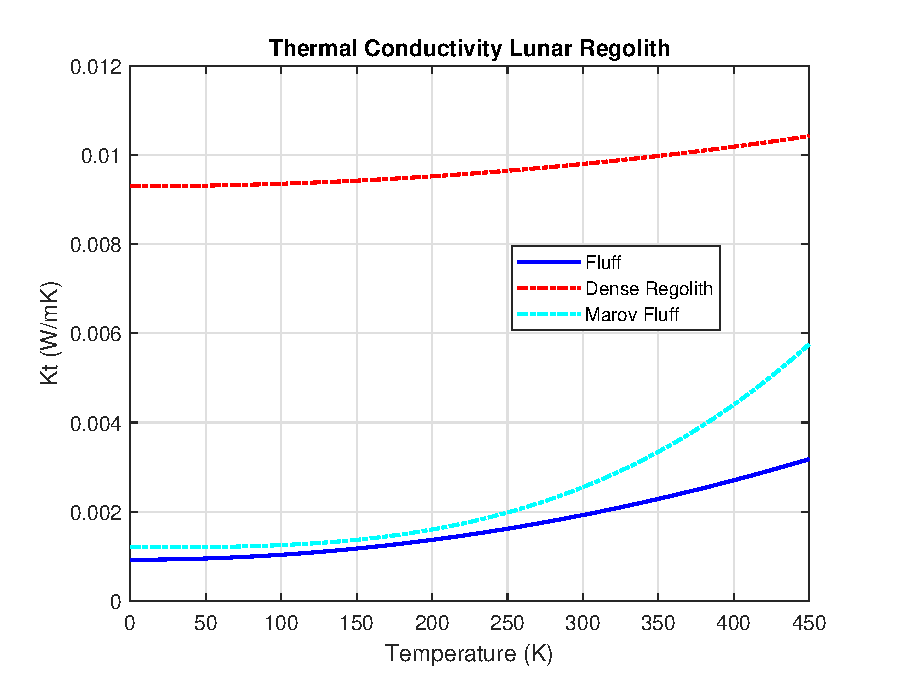
\includegraphics[width=.9\textwidth]{thermal_conductivity.eps}   
      \end{center}  

\end{frame}

\begin{frame}{Heat Capacity}
The heat capacity is found from the bulk thermal inertia, $I = 0.019 m^2 s^{1/2} \frac{K}{J}$ which is set equal to the inverse root of the thermal conductivity, density, and heat capacity \cite{Racca}. 
\begin{align*}
I & = \frac{1}{\sqrt{K_t \rho C_v}} \quad \text{Solving for $C_v$	}\\
C_v & = \frac{1}{K_t \rho I^2}
\end{align*}
Where we tale the density of the regolith to be $ 1900 \frac{Kg}{m^3} $  and the fluff at $1300\frac{Kg}{m^3} $\cite{Malla}.
\end{frame}






%
%\begin{frame}{Temperature dampening due to regolith layers }
%For a temperature on the surface, $z = 0$, varied with time,
%\begin{align*}
%\theta(0,t) & = \theta_{avg}+\theta_0 cos(\omega t)
%\end{align*} 
%Where $\theta_0$ is half the difference between the high and low temperatures, and $\theta_{avg}$ is the average of the high and low.
% 
%\end{frame}



  
\begin{frame}{Temperature dampening due to regolith layers }
As layers of `fluff' regolith insulation surrounding the habitat increase less heat is diffused to the structure.  
We can find the characteristic penetration depth from the thermal diffusivity and omega,
\begin{align*}
\delta & = \sqrt{\frac{D_t}{\omega}}
\end{align*}
Where $D_t = \frac{K_t}{C_v}$

\end{frame}




  
\begin{frame}{Temperature dampening due to regolith layers }
We can simulate a temperature pulse through the depth of surface over time to estimate the depth needed to minimize temperature fluctuations,
\begin{align*}
\theta(z,t) & = \theta_{avg}+\theta_0 e^{\frac{-z}{\delta}} cos(\omega t- \frac{z}{\delta})
\end{align*}

\end{frame}





\begin{frame}{Matlab Functions}
 Matlab functions were written to generate numerical values for the thermal conductivity, which are used to find the heat capacity from the thermal inertial and density where we can then find the penetration depth. A Temperature pulse can then be simulated.
\end{frame}

\begin{frame}{ Dense Regolith}
The denser regolith layer shows strong thermal conductivity. This layer can be used for heat and energy storage or to dissipate heat from solar panels.
 \begin{center}
             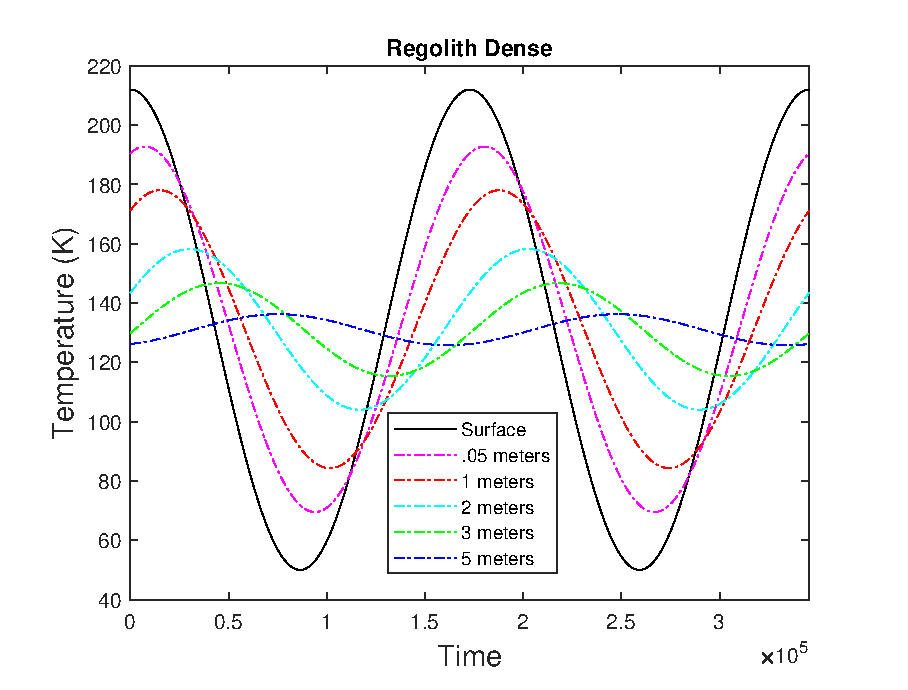
\includegraphics[width= .75\textwidth]{Regolith_Pulse.eps}   
      \end{center}  
\end{frame}


\begin{frame}{Fluff Regolith}
A loose mixture of the top 'fluff' layer of lunar regolith  which has a lower thermal conductivity and thus higher thermal shielding can be used as a strong insulator\cite{Malla}.
 \begin{center}
             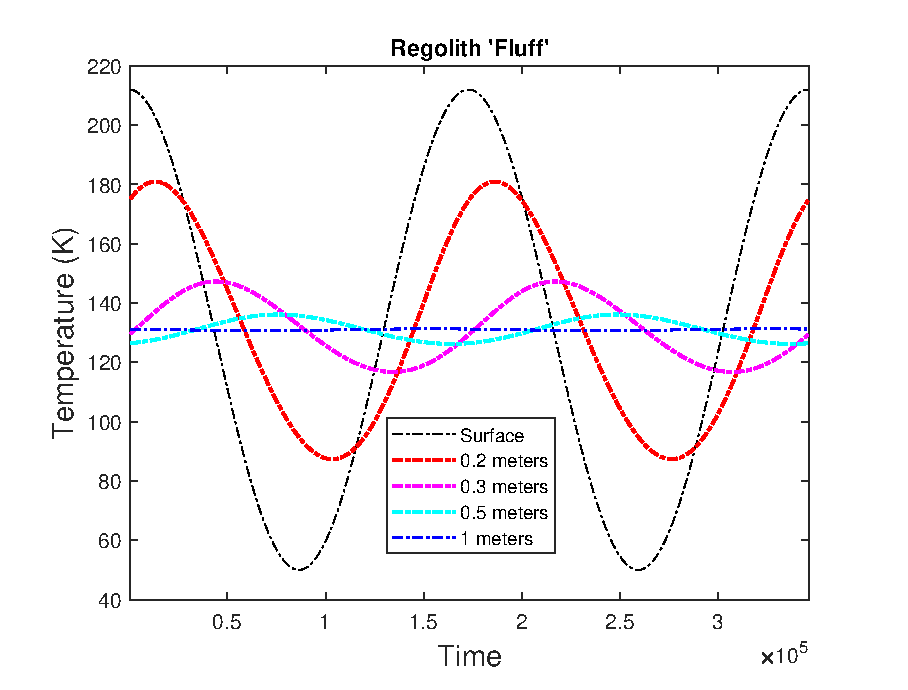
\includegraphics[width= .75\textwidth]{Processed_Regolith.eps}   
      \end{center}  
\end{frame}


\begin{frame}{Using Lunar Regolith as Insulation}
Since lunar regolith, (layers of dust and rock), is abundant on the surface any material use of it  alleviates the need to import another substance. By using the regolith as a insulative material it may be possible to minimize the temperature variations inside the habitat and create a steady state temperature environment that could then be heated at a constant rate.
 \begin{center}
             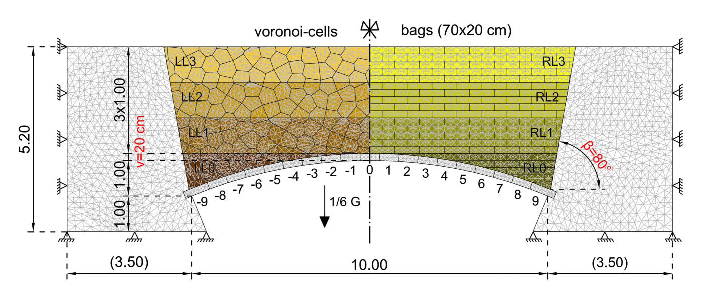
\includegraphics[width=.75\textwidth]{bags.eps}   
      \end{center}  

\end{frame}



\begin{thebibliography}{99}
% The numeral (here 99) in curly braces is nominally the number of entries in
% the bibliography. It's supposed to affect the amount of space around the
% numerical labels, so only the number of digits should matter--and even that
% seems to make no discernible difference.



\bibitem{Koebel}David Koebel, Michele Bonerba, Daniel Behrenwaldt, Matthias Wieser, Carsten Borowy,
Analysis of landing site attributes for future missions targeting the rim of the lunar South Pole Aitken basin,
Acta Astronautica,
Volume 80,
2012,
Pages 197-215

\bibitem{Yao}Xiaochen Lu, Wei Yao, Chao Wang, Rong Ma,
Exergy analysis of a lunar based solar thermal power system with finite-time thermodynamics,
Energy Procedia,
Volume 158,
2019,
Pages 792-796


\bibitem{Belz} Belz et al., 2011. Hybrid life support systems with integrated fuel cells and photobioreactors for a lunar base. Aerospace Science and Technology, pp.Aerospace Science and Technology.

\bibitem{Hickman}Hickman, J.M., Curtis, H.B. \& Landis, G., 1990. Design considerations for lunar base photovoltaic power systems, Washington, DC] : [Springfield, Va.]: National Aeronautics and Space Administration

\bibitem{Climent}Blai Climent, Oscar Torroba, Ricard González-Cinca, Narayanan Ramachandran, Michael D. Griffin,
Heat storage and electricity generation in the Moon during the lunar night,
Acta Astronautica,
Volume 93,
2014,
Pages 352-358

\bibitem{Heldmann}Jennifer L. Heldmann, et al. Site selection and traverse planning to support a lunar polar rover mission: A case study at Haworth Crater,
Acta Astronautica, Volume 127, 2016, Pages 308-320,

\bibitem{Toth}Toth, A.R. \& Bagi, K., 2011. Analysis of a Lunar Base Structure Using the Discrete-Element Method. Journal Of Aerospace Engineering, 24(3), pp.397–401.

\bibitem{Williams}J.P. Williams, D.A. Paige, B.T. Greenhagen, E. Sefton-Nash,
The global surface temperatures of the Moon as measured by the Diviner Lunar Radiometer Experiment,
Icarus,
Volume 283,
2017,
Pages 300-325


\bibitem{Vasavada}A.R.Vasavada,D.A.Paige,S.E.Wood,Near surface temperatures on
mercury and the moon and the stability of polar ice deposits,Icarus
141(1999)179–193.

\bibitem{Racca}G. Racca,Moon surface thermal characteristics for moon orbiting
spacecraft thermal analysis,Planet.SpaceSci.43(1983)835–842.

\bibitem{Malla}Ramesh B. Malla, Kevin M. Brown,
Determination of temperature variation on lunar surface and subsurface for habitat analysis and design,
Acta Astronautica,
Volume 107,
2015,
Pages 196-207

\bibitem{Hayne}Hayne et al., 2015. Evidence for exposed water ice in the Moon’s south polar regions from Lunar Reconnaissance Orbiter ultraviolet albedo and temperature measurements. Icarus, 255, pp.58–69.


\bibitem{Liebert}Curt H. Liebert und Russell E. Hurt, Jr. SOLAR CELL PERFORMANCE
AT LOW TEMPERATURES AND
SIMULATED SOLAR INTENSITIES
NATIONAL AERONAUTICS AND SPACE ADMINISTRATION

\bibitem{Mcevoy}Mcevoy, A 2011, Practical Handbook of Photovoltaics : Fundamentals and Applications, Elsevier Science \& Technology, San Diego..

\bibitem{Mazarico}E. Mazarico, G.A. Neumann, D.E. Smith, M.T. Zuber, M.H. Torrence,
Illumination conditions of the lunar polar regions using LOLA topography,
Icarus,
Volume 211, Issue 2,
2011,
Pages 1066-1081


\bibitem{Bussey}D.B.J. Bussey, J.A. McGovern, P.D. Spudis, C.D. Neish, H. Noda, Y. Ishihara, S.A. Sorensen,
Illumination conditions of the south pole of the Moon derived using Kaguya topography,
Icarus,
Volume 208, Issue 2,
2010,
Pages 558-564

\end{thebibliography}


\end{document}